\documentclass{article}

\usepackage{graphicx}
\usepackage{apacite}                      % to use apa citation style

\begin{document}

\tableofcontents                          % add table of contents automatically
\newpage

% \begin{figure}[h!]                      % use h to insert plot at the exact place
\begin{figure}
  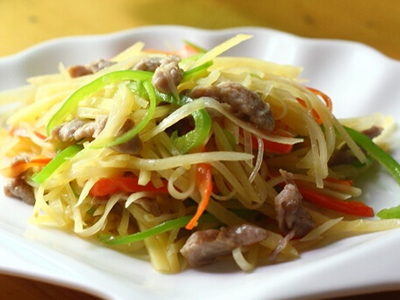
\includegraphics[width=\linewidth]{hungry.jpg}
  \caption{show some food}
  \label{fig:food1}                       % can be used by ref in later content (see below for example) 
\end{figure}

\section{Food topic}

BLABLABLA

\subsection{Food example}

Food intro. Figure \ref{fig:food1} shows how hungry I was at the moment of making this doc.


\begin{table}[h!]                       % add a fake table
  \caption{Dummy table}
\end{table}
...\\
Please find my trial citation \cite{ROGERS:2010} in this text.   \par

This is some example text\footnote{\label{myfootnote}Hello there!}. \par         % add footnote
I'm referring to footnote \ref{myfootnote}.

\newpage
\begin{appendix}                        % add appendix of plots and tables in new page
  \listoffigures
  \listoftables
\end{appendix}


\newpage
\bibliographystyle{apacite}             % use APA style citation
% \bibliographystyle{ieeetr}
% \bibliographystyle{apalike}
\bibliography{tryref}                   % use the reference in txt file tryref.bib
% w: try delete .aux file if not work
% w: wait until the pkg is successfully installed !!




\end{document}